\chapter{Resultados}

Neste capítulo, será apresentada a ferramenta obtida, assim como detalhes sobre o tempo de execução.

\section[Ferramenta]{Ferramenta}

A ferramenta desenvolvida atua a partir de uma gravação no plano coronal da execução do movimento de barra fixa, processando a imagem de modo a detectar a barra e os pontos de referência do corpo humano. Logo em seguida, ocorre a segmentação da imagem e cálculos algébricos, retornando o estado atual do movimento de barra fixa e dados sobre o movimento como forma de feedback. Todo esse processo segue o fluxograma abaixo.

\begin{figure}[H]
	\centering
  \caption{Fluxograma do processo executado pela ferramenta.}
	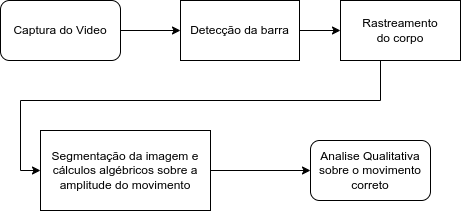
\includegraphics[scale=0.7]{figuras/diagrama/processo.png}
  \legend{Fonte: Elaborado pelo autor (2023)}
	\label{fig:fluxo}
\end{figure}


\section[Parte Gráfica]{Parte Gráfica}

A parte gráfica da ferramenta é baseada em duas telas: a tela de exibição, que se assemelha a um player e é responsável exclusivamente por exibir o vídeo e as informações referentes ao feedback, e o painel de controle, que é destacado do player. No entanto, sua única função é controlar o que será exibido no player.

\begin{figure}[H]
	\centering
	\caption{Tela \aspas{player}}
	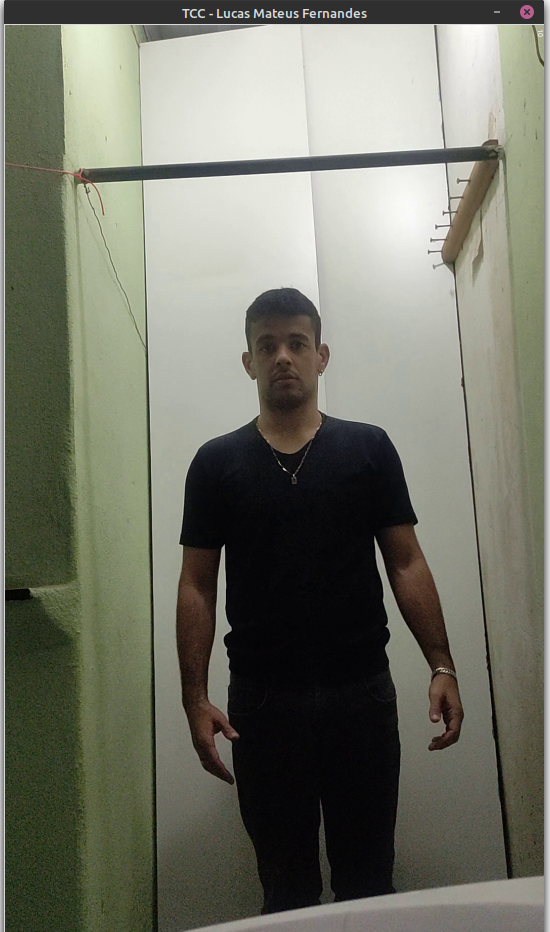
\includegraphics[scale=0.25]{figuras/view/player.png}
	\legend{Fonte: Elaborado pelo autor (2023)}
\end{figure}


A tela responsável por ser um painel de controle do player possui nove campos de entrada, sendo duas caixas de texto \aspas{Speed} e \aspas{Frame}, e cinco botões: \aspas{PLAY}, \aspas{SaveF}, \aspas{SaveV}, \aspas{Barra}, \aspas{Dados}, \aspas{EPH}, e uma barra deslizante.

\begin{figure}[H]
	\centering
	\caption{Tela \aspas{painel de controle}}
	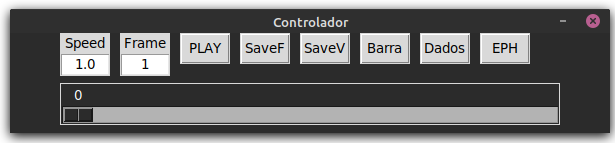
\includegraphics[scale=0.5]{figuras/view/painel_controller.png}
	\legend{Fonte: Elaborado pelo autor (2023)}
\end{figure}


\begin{itemize}
	\item A caixa de texto \aspas{Speed} recebe um número decimal como entrada, representando um escalar pelo qual a velocidade de reprodução será alterada;

	\item A caixa de texto \aspas{Frame} recebe um número inteiro como entrada, movendo o vídeo para o \textit{frame} semelhante à barra deslizante que altera o \textit{frame} em exibição;
	
	\item O botão \aspas{PLAY} é responsável por reproduzir e pausar o vídeo;
	
	\item O botão \aspas{SaveF} salva o \textit{frame} visualizado no diretório \aspas{./midia/dist} do projeto;
	
	\item O botão \aspas{SaveV} realiza a mesma ação do \aspas{SaveF}, mas para um vídeo em vez de uma imagem;
	
	\item O botão \aspas{Barra} destaca a posição da barra no vídeo;
	
	\item O botão \aspas{EPH} destaca a pose do executor traçando segmentos de reta sobre os membros e o tronco;
    
    \item O botão \aspas{Dados} exibe informações no canto superior esquerdo, como o ID do \textit{frame}, o estado do \ac{AFD}, a quantidade de barras realizadas, o ângulo entre o braço e antebraço, o ângulo formado pela perna e coxa, o ângulo pelo qual o vídeo foi rotacionado para a barra ficar paralela ao solo, condições como: se a mão está tocando a barra, se o cotovelo está estendido ou flexionado, se as pernas estão dobradas, se a cabeça ultrapassou a barra, a distância do peito até a barra, se o peito tocou a barra e o caractere do \ac{AFD} que representa o \textit{frame} atual.
	
\end{itemize}



\begin{figure}[H]
	\centering
	\caption{Resultado final com todas as Flags ativas \aspas{Barra}, \aspas{Dados} e \aspas{EPH}}
	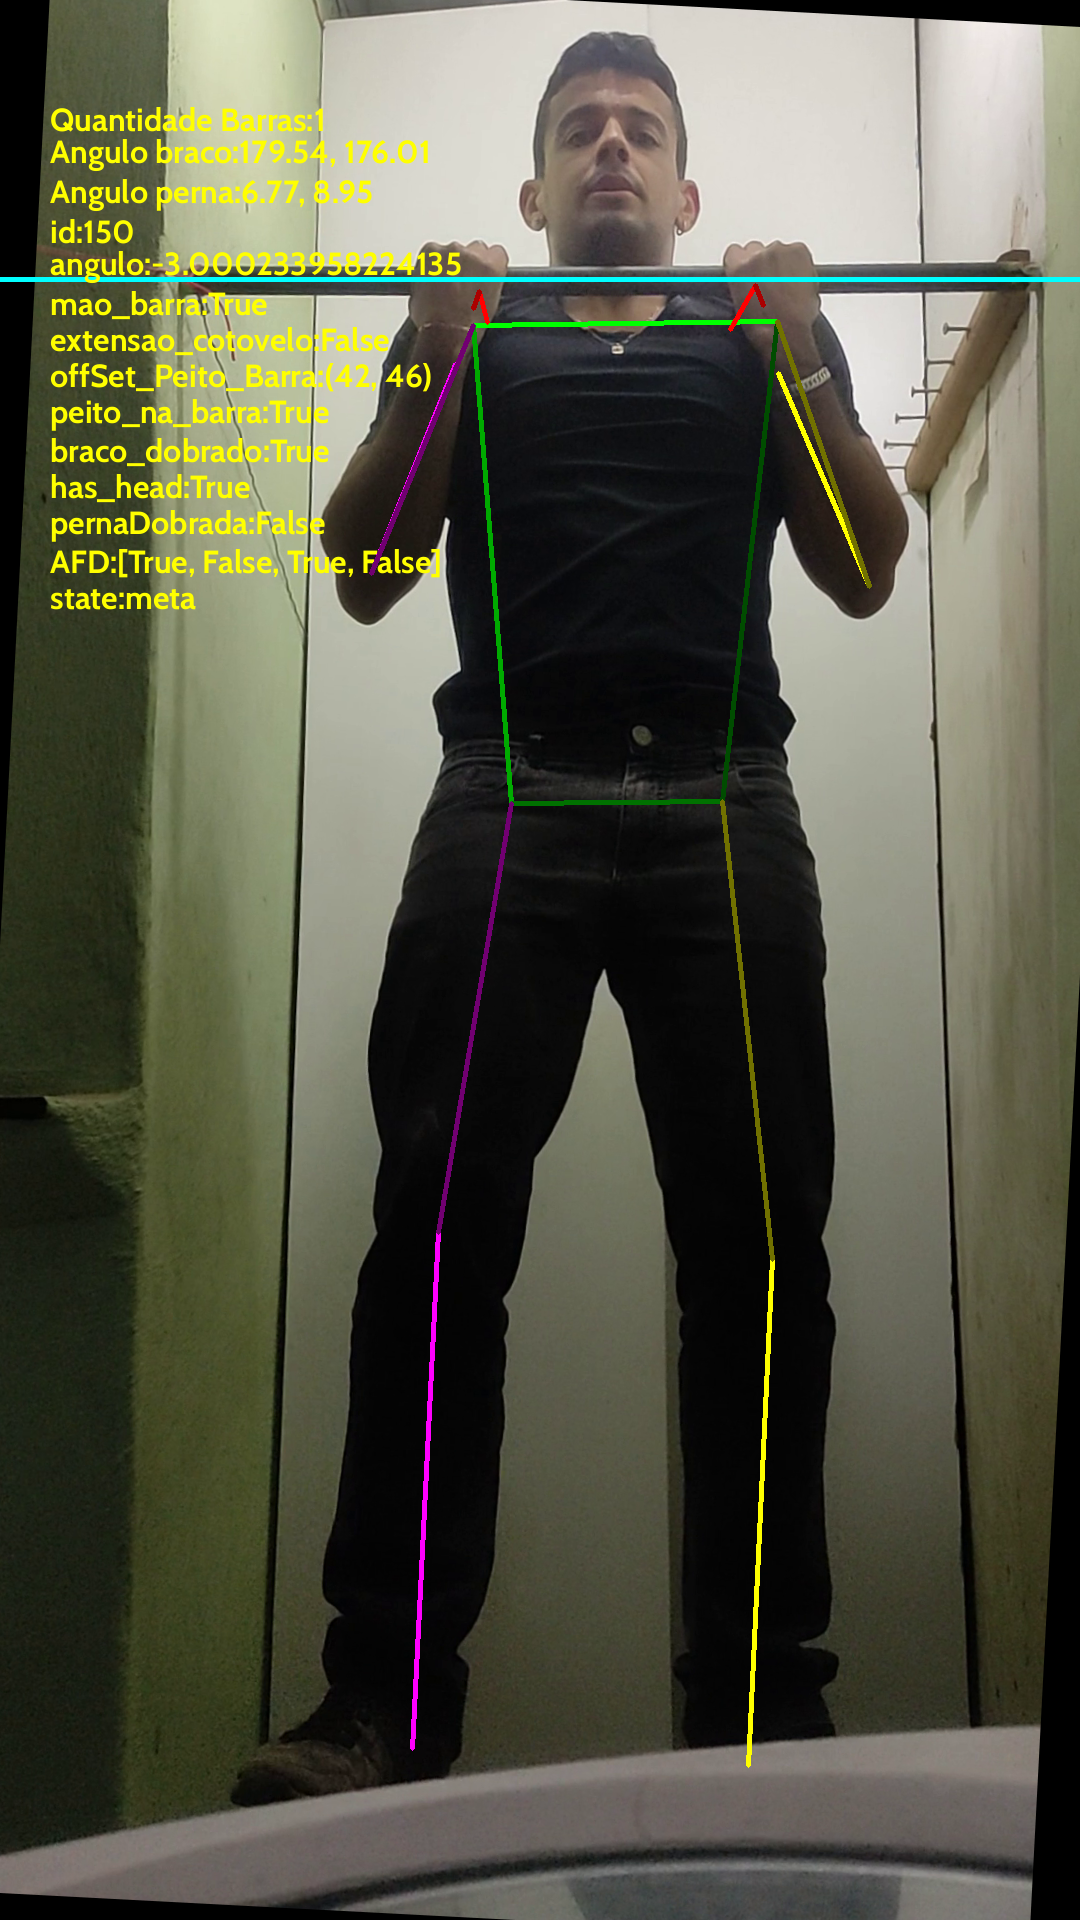
\includegraphics[scale=0.2]{figuras/flags.png}
	\legend{Fonte: Elaborado pelo autor (2023)}
\end{figure}



\section[Tempo de execução]{Tempo de execução}

O tempo de execução desempenha um papel crucial, pois representa o intervalo de tempo necessário para que um programa ou algoritmo conclua uma tarefa específica. É um fator fundamental na avaliação e otimização de sistemas computacionais, utilizado como métrica para comparar a eficiência de diferentes abordagens e soluções, buscando identificar a estratégia mais eficaz para realizar uma tarefa determinada. Portanto, para os testes, foi avaliado um vídeo de 211 frames a uma taxa de 24 frames por segundo, realizando uma execução correta do movimento de barra fixa. Para a amostragem, foram realizadas 10 iterações da execução do programa.


\newpage
Para um melhor entendimento dos resultados, o processamento de um frame foi denominado de \aspas{process\_cell} e é subdividido em funções, sendo elas:

\begin{itemize}
	\item Função \aspas{barra} responsável pela Detecção da barra, conforme demonstrado na seção \ref{sec:Deteccao da barra};
	\item Função \aspas{verify\_inclination} responsável pela rotação da imagem de acordo com a inclinação da barra, conforme demonstrado na seção \ref{sec:Inclinacao da barra};
	\item Função \aspas{verify\_eph} responsável pela identificação dos pontos chaves do corpo humano, conforme demonstrado na seção \ref{sec:Reconhecimento de pose humana};
	\item Função \aspas{verify\_angle\_member} responsável pela identificação dos ângulos entre os segmentos, conforme demonstrado na seção \ref{angulo_braco} e \ref{sec:Movimentacao do quadril}; 
	\item Função \aspas{verify\_char\_AFD} responsável pela extração das informações presentes no caractere do \ac{AFD}, conforme explicado em \ref{sec:Estrategia para deteccao do movimento correto de barra fixa}. Sendo um compilado de quatro funções.
		
	\begin{itemize}
		
		\item Função \aspas{verify\_maoBarra} responsável pela verificação do contato da mão com a barra, demonstrado na seção \ref{sec:Mao na barra};
		\item Função \aspas{verify\_extensaoCotovelo} responsável pela verificação da extensão do braço, demonstrado na seção \ref{sec:Braco esticado};
		\item Função \aspas{verify\_ultrapassarBarra} responsável pela verificação da ultrapassagem do queixo à barra, demonstrado na seção \ref{sec:meta};
		\item Função \aspas{verify\_movimentoQuadrilPerna} responsável pela verificação da flexão dos membros inferiores, demonstrado na seção \ref{sec:Movimentacao do quadril}.

	\end{itemize}

	\item Função \aspas{verify\_AFD} responsável pela computação do \ac{AFD}, demonstrado na seção \ref{fig:transicaoAFD}.

\end{itemize}

% Os gráficos presentes nas figuras \ref{graf:G1} \ref{graf:G2} \ref{graf:G3} \ref{graf:G4} \ref{graf:G5} \ref{graf:G6} \ref{graf:G7} \ref{graf:G8} \ref{graf:G9} \ref{graf:G10} \ref{graf:G11} mostram no eixo vertical o tempo gasto em segundos para o processamento da função, associado aos identificadores dos frames representado no eixo horizontal, com  base em dados proveniente de 10 iterações.




% \begin{figure}[H]
% 	\centering
% 	\caption{Tempo de execução da função \aspas{barra} em 10 iterações mostrando a média, mínimo e máximo do tempo gasto por quadro em segundos}
% 	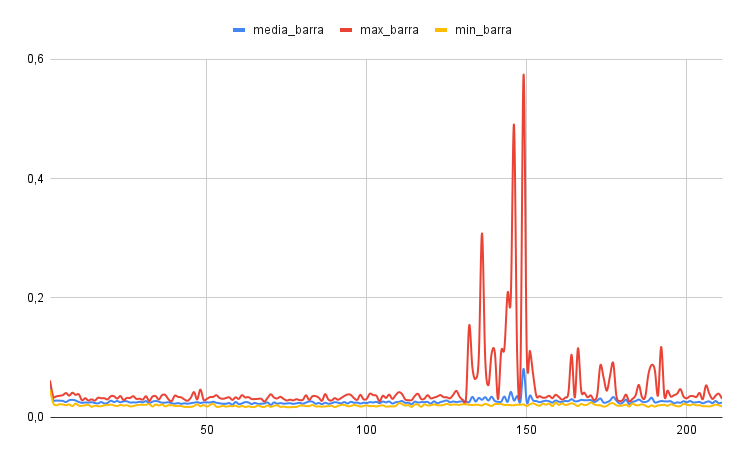
\includegraphics[scale=0.5]{figuras/grafico/barra.png}
% 	\label{graf:G1}
% 	\legend{Fonte: Elaborado pelo autor (2023)}
% \end{figure}

% \begin{figure}[H]
% 	\centering
% 	\caption{Tempo de execução da função \aspas{verify\_inclination} em 10 iterações mostrando a média, mínimo e máximo do tempo gasto por quadro em segundos}
% 	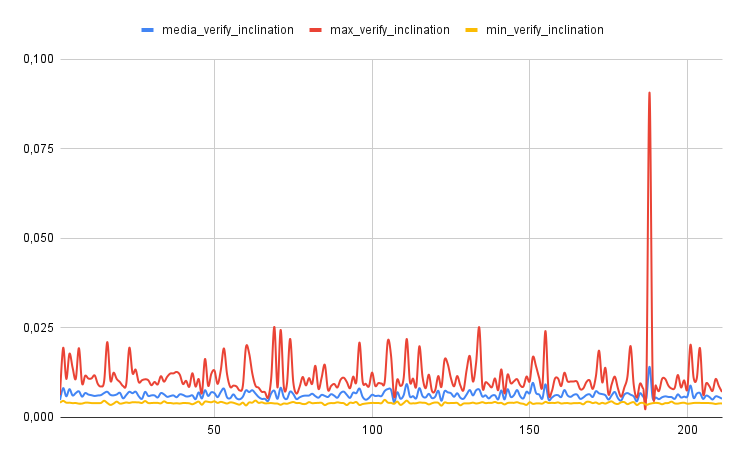
\includegraphics[scale=0.5]{figuras/grafico/inclination.png}
% 	\label{graf:G2}
% 	\legend{Fonte: Elaborado pelo autor (2023)}
% \end{figure}


% \begin{figure}[H]
% 	\centering
% 	\caption{Tempo de execução da função \aspas{verify\_eph} em 10 iterações mostrando a média, mínimo e máximo do tempo gasto por quadro em segundos}
% 	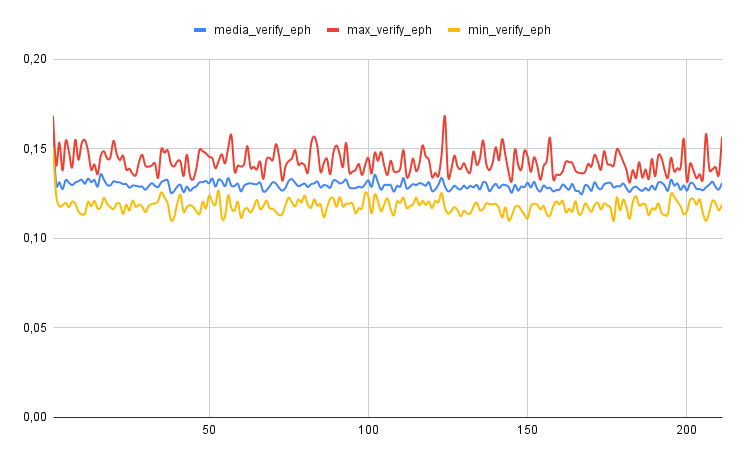
\includegraphics[scale=0.5]{figuras/grafico/eph.png}
% 	\label{graf:G3}
% 	\legend{Fonte: Elaborado pelo autor (2023)}
% \end{figure}


% \begin{figure}[H]
% 	\centering
% 	\caption{Tempo de execução da função \aspas{verify\_angle\_member} em 10 iterações mostrando a média, mínimo e máximo do tempo gasto por quadro em segundos}
% 	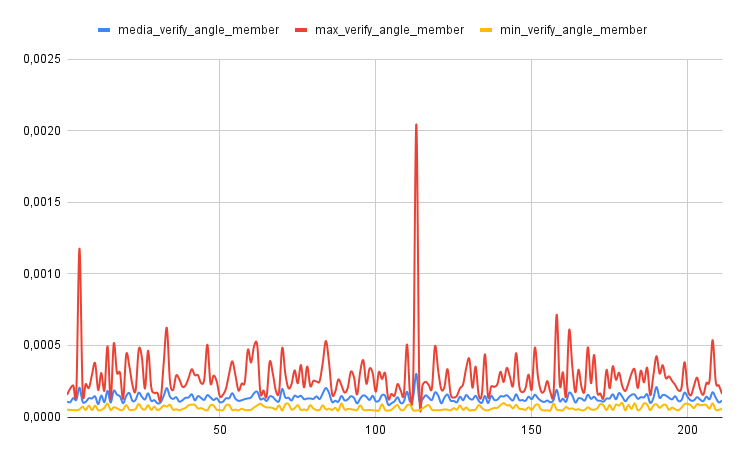
\includegraphics[scale=0.6]{figuras/grafico/angulo.png}
% 	\label{graf:G4}
% 	\legend{Fonte: Elaborado pelo autor (2023)}
% \end{figure}


% \begin{figure}[H]
% 	\centering
% 	\caption{Tempo de execução da função \aspas{verify\_char\_AFD} em 10 iterações mostrando a média, mínimo e máximo do tempo gasto por quadro em segundos}
% 	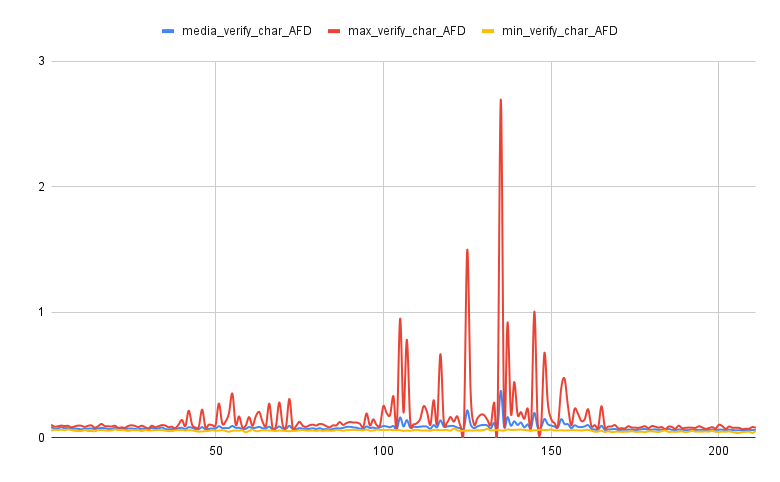
\includegraphics[scale=0.55]{figuras/grafico/char_AFD.png}
% 	\label{graf:G5}
% 	\legend{Fonte: Elaborado pelo autor (2023)}
% \end{figure}



% \begin{figure}[H]
% 	\centering
% 	\caption{Tempo de execução da função \aspas{verify\_maoBarra} em 10 iterações mostrando a média, mínimo e máximo do tempo gasto por quadro em segundos}
% 	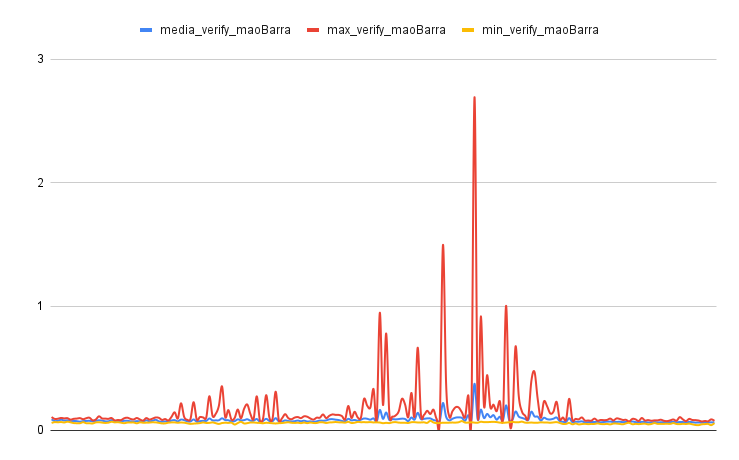
\includegraphics[scale=0.45]{figuras/grafico/maoBarra.png}
% 	\label{graf:G6}
% 	\legend{Fonte: Elaborado pelo autor (2023)}
% \end{figure}


% \begin{figure}[H]
% 	\centering
% 	\caption{Tempo de execução da função \aspas{verify\_extensaoCotovelo} em 10 iterações mostrando a média, mínimo e máximo do tempo gasto por quadro em segundos}
% 	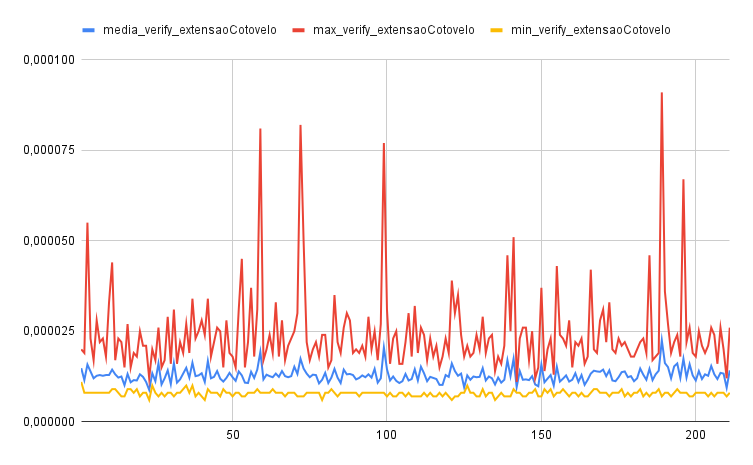
\includegraphics[scale=0.45]{figuras/grafico/extensaoCotovelo.png}
% 	\label{graf:G7}
% 	\legend{Fonte: Elaborado pelo autor (2023)}
% \end{figure}


% \begin{figure}[H]
% 	\centering
% 	\caption{Tempo de execução da função \aspas{verify\_ultrapassarBarra} em 10 iterações mostrando a média, mínimo e máximo do tempo gasto por quadro em segundos}
% 	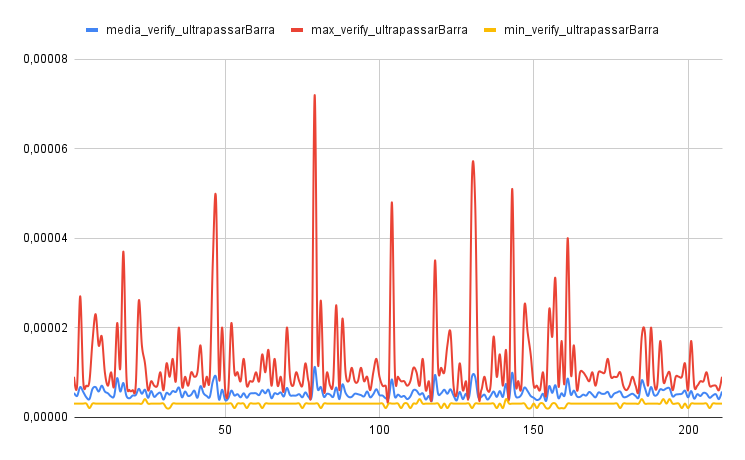
\includegraphics[scale=0.55]{figuras/grafico/ultrapassarBarra.png}
% 	\label{graf:G8}
% 	\legend{Fonte: Elaborado pelo autor (2023)}
% \end{figure}


% \begin{figure}[H]
% 	\centering
% 	\caption{Tempo de execução da função \aspas{verify\_movimentoQuadrilPerna} em 10 iterações mostrando a média, mínimo e máximo do tempo gasto por quadro em segundos}
% 	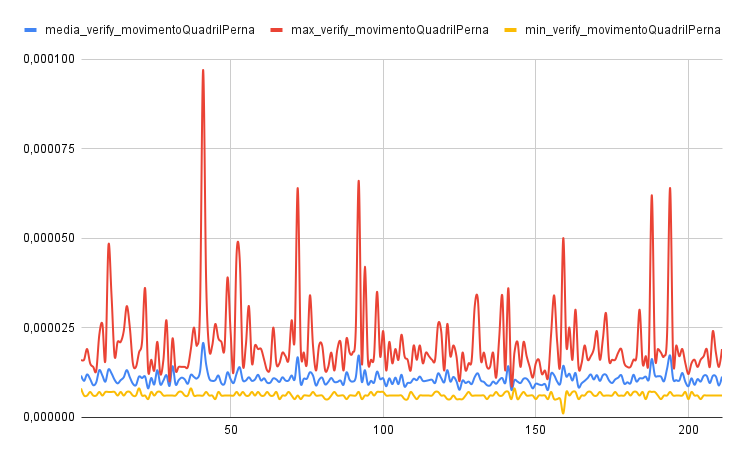
\includegraphics[scale=0.55]{figuras/grafico/movimentoQuadril.png}
% 	\label{graf:G9}
% 	\legend{Fonte: Elaborado pelo autor (2023)}
% \end{figure}


% \begin{figure}[H]
% 	\centering
% 	\caption{Tempo de execução da função \aspas{verify\_AFD} em 10 iterações mostrando a média, mínimo e máximo do tempo gasto por quadro em segundos}
% 	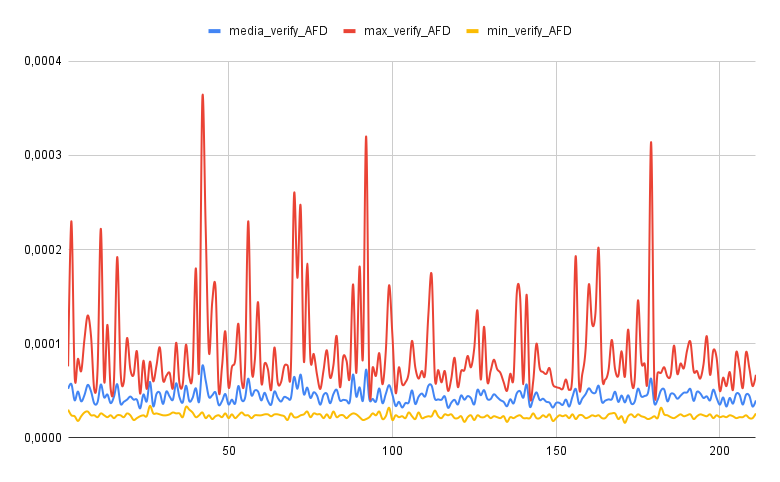
\includegraphics[scale=0.55]{figuras/grafico/verify_AFD.png}
% 	\label{graf:G10}
% 	\legend{Fonte: Elaborado pelo autor (2023)}
% \end{figure}


% \begin{figure}[H]
% 	\centering
% 	\caption{Tempo de execução da função \aspas{process\_cell} em 10 iterações mostrando a média, mínimo e máximo do tempo gasto por quadro em segundos}
% 	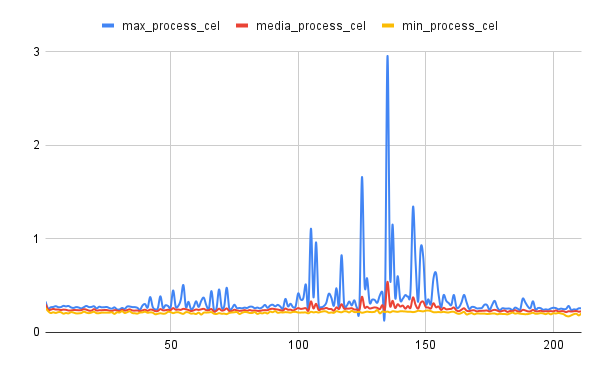
\includegraphics[scale=0.8]{figuras/grafico/process_cell.png}
% 	\label{graf:G11}
% 	\legend{Fonte: Elaborado pelo autor (2023)}
% \end{figure}



A função \aspas{verify\_char\_AFD} é responsável pela extração das informações para a criação do caractere do AFD e é composta pelas funções \aspas{verify\_maoBarra}, \aspas{verify\_extensaoCotovelo}, \aspas{verify\_ultrapassarBarra} e \aspas{verify\_movimentoQuadrilPerna}. Entre as funções que a compõem, \aspas{verify\_maoBarra} se destaca por gastar cerca de 99,09\% do tempo de processamento em relação ao tempo gasto por \aspas{verify\_char\_AFD}.


O gráfico da Figura \ref{graf:G13} apresenta, com base em 10 iterações, a média do tempo gasto em segundos por cada função que compõe a função \aspas{process\_cell}. No eixo vertical, é demonstrado o tempo gasto em uma escala de 0,1 segundos, enquanto no eixo horizontal são representados os identificadores dos frames, variando de 1 a 211. Devido à escala de 0,1 segundos, algumas funções não são visíveis no gráfico, uma vez que estão em uma escala relativamente pequena em comparação com a escala de 0,1 segundos.

\begin{figure}[H]
	\centering
	\caption{Tempo médio de execução das funções que compõe \aspas{process\_cell}}
	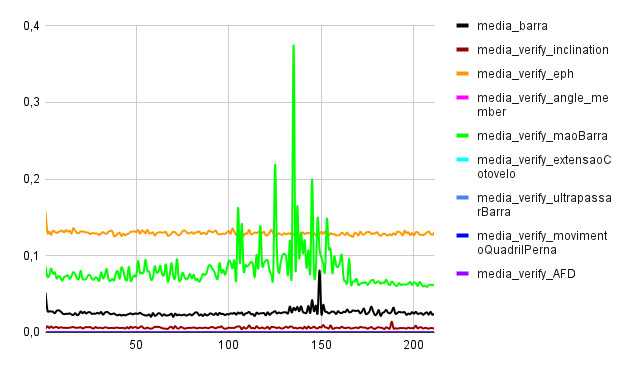
\includegraphics[scale=0.7]{figuras/grafico/comp_process_cell_2.png}
	\label{graf:G13}
	\legend{Fonte: Elaborado pelo autor (2023)}
\end{figure}


O gráfico da figura \ref{graf:G14} mostra o desempenho relativo de cada função que compõe \aspas{process\_cell} em relação a própria função \aspas{process\_cell}

\begin{figure}[H]
	\centering
	\caption{Média de 10 iterações do percentual de tempo gasto por cada função associado ao processamento de um frame}
	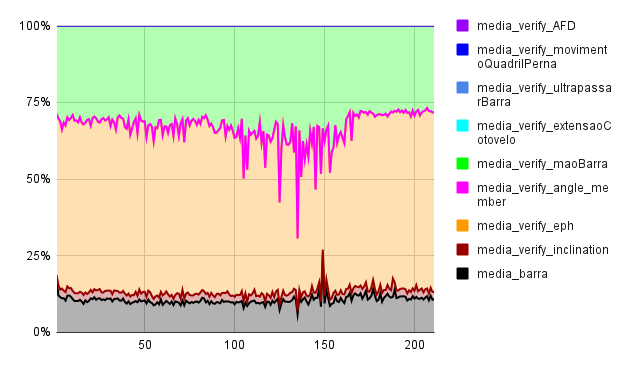
\includegraphics[scale=0.7]{figuras/grafico/comp_process_cell_1.png}
	\label{graf:G14}
	\legend{Fonte: Elaborado pelo autor (2023)}
\end{figure}

As duas funções mais relevantes para a alta taxa de latência do processamento do frame são \aspas{verify\_eph} e \aspas{verify\_maoBarra}, sendo responsáveis por cerca de 85,14\% do tempo gasto por \aspas{process\_cell}.

\begin{table}[H]
	\centering
	\begin{tabular}{|p{6cm}|p{3cm}|p{5cm}|}
	\hline
	\textbf{Função} & \textbf{Tempo médio em segundos} & \textbf{Menor tempo registrado em segundos} \\
	\hline
	barra & 0,03422 & 0,016335 \\
	verify\_inclination & 0,00603 & 0,00317 \\
	verify\_eph & 0,1293617 & 0,109623 \\
	verify\_angle\_member & 0,00013 & 0,000045 \\
	verify\_char\_AFD & 0,0753571 & 0,039386 \\
	verify\_AFD & 0,0000427 & 0,000016 \\
	\hline
	\end{tabular}
	\caption{Tempos médios e menores tempos registrados para cada função que compõe process\_cell}
	\label{tab:tempos_funcoes}
\end{table}



\begin{table}[H]
	\centering
	\begin{tabular}{|p{6cm}|p{3cm}|p{5cm}|}
	\hline
	\textbf{Função} & \textbf{Tempo médio em segundos} & \textbf{Menor tempo registrado em segundos} \\
	\hline
	verify\_maoBarra & 0,0747025 & 0,03924 \\
	verify\_extensaoCotovelo & 0,0000126 & 0,000006  \\
	verify\_ultrapassarBarra & 0,0000051 & 0,000002  \\
	verify\_movimentoQuadrilPerna & 0,0000104 & 0,000001  \\
	\hline
	\end{tabular}
	\caption{Tempos médios e menores tempos registrados para cada função que compõe verify\_char\_AFD}
	\label{tab:tempos_funcoes_especificas}
\end{table}
		
Por fim, o tempo médio para a execução da função \aspas{process\_cell} foi de 0,2481895403 segundos, enquanto o menor tempo registrado foi de 0,171841 segundos, assumindo um desvio padrão de 0,03161229806 e uma variância de 0,0009993373889.
